\documentclass[11pt,a4paper]{article}

\usepackage[utf8]{inputenc}
\usepackage[T1]{fontenc}
\usepackage[spanish,es-nodecimaldot]{babel}
\usepackage{lmodern}
\usepackage{geometry}
\usepackage{booktabs}
\usepackage{tabularx}
\usepackage{array}
\usepackage{enumitem}
\usepackage{hyperref}
\usepackage{float}
\usepackage{amsmath}
\usepackage{graphicx}
\graphicspath{{figures/}}
\usepackage[font=small, labelfont=bf]{caption}
\setlist[itemize]{label=\textbullet}

\geometry{top=2.3cm, bottom=2.3cm, left=2.4cm, right=2.4cm}
\hypersetup{colorlinks=true, urlcolor=blue, linkcolor=black}

\setlength{\parindent}{0pt}
\setlength{\parskip}{0.6em}
\renewcommand{\arraystretch}{1.2}
\urlstyle{same}

\newcolumntype{Y}{>{\raggedright\arraybackslash}X}
\newcolumntype{R}{>{\raggedleft\arraybackslash}X}
\newcommand{\code}[1]{\texttt{\small #1}}

\title{
    \textbf{Exploración de modelos de Inteligencia Artificial multimodal\\
    para la identificación de macromicetos mediante dispositivos móviles}\\[0.6em]
    \normalsize Resultados de las Semanas 5 y 6: modelo para celular, resultados por nivel taxonómico y orden del código
}

\author{
    Daniel Esteban Camacho Ospina\\
    Cesar Augusto Pulido Cuervo
}

\date{}

\begin{document}

\maketitle

% =========================================================
\section{Objetivo}
% =========================================================

\begin{itemize}[leftmargin=*]
    \item \textbf{Semana 5:} entrenar un modelo liviano que pueda funcionar en un
    celular, ajustar su configuración y tratar el desequilibrio entre géneros.
    \item \textbf{Semana 6:} medir los resultados no solo por género sino también
    por familia, orden, clase y filo, y ordenar el código para la Fase 5.
\end{itemize}

Todo usa la versión \code{v002} del dataset: solo FungiTastic, los mismos diez
géneros y las particiones oficiales (17\,799 observaciones para entrenar,
3\,452 para validar y 4\,039 para la prueba final). Una \emph{observación} es un
hongo encontrado por una persona; puede tener varias fotos. Los resultados
principales se dan por observación.

La métrica principal es el \textbf{F1 promedio por género}: para cada género se
combina qué tanto acierta cuando lo nombra y qué tanto lo encuentra, y luego se
promedia dando el mismo peso a los diez géneros. Así un género con pocas fotos
cuenta igual que uno con muchas. Va de 0 a 1.

Las decisiones se toman solo con \textbf{validación}. La \textbf{prueba} se usa
una sola vez al final, para que el resultado no esté influido por los ajustes.

% =========================================================
\section{Semana 5: modelo para celular}
% =========================================================

\subsection{Modelo elegido}

Se comparó el modelo de referencia de la Semana 4 (ResNet-18) con
\textbf{MobileNetV3-Large}, diseñado para celulares. Ambos parten de redes ya
entrenadas con millones de imágenes generales y se reajustan con fotos de hongos.

\begin{figure}[H]
\centering
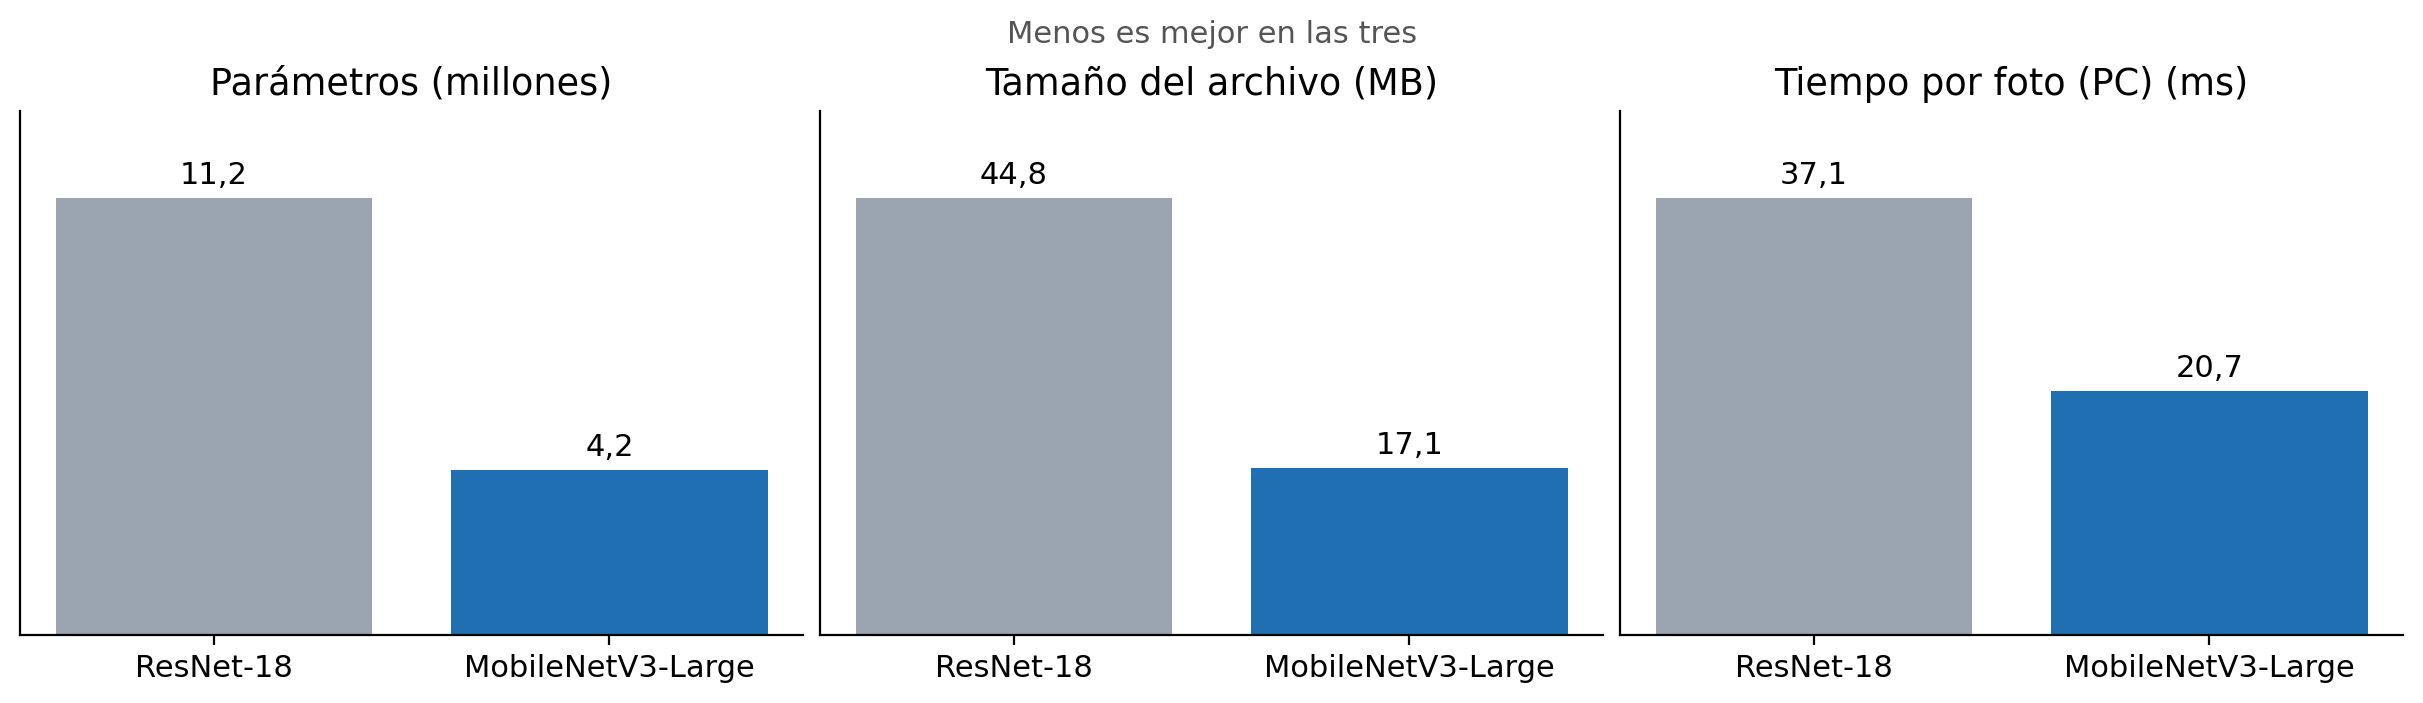
\includegraphics[width=\textwidth]{s5_s6_size_speed.png}
\caption{Tamaño y velocidad de los dos modelos (\code{reports/s5/architecture\_profile.json}).}
\end{figure}

MobileNet es un 62\,\% más pequeño y casi el doble de rápido. El tiempo se midió
en el procesador del PC, \textbf{no en un celular}; falta medirlo en Android.

\subsection{Configuración del ensayo A}

\begin{table}[H]
\centering
\small
\begin{tabularx}{\textwidth}{Y l}
\toprule
\textbf{Ajuste} & \textbf{Valor}\\
\midrule
Velocidad de aprendizaje (qué tan grandes son los ajustes en cada paso) & 0,0003\\
Fotos por paso & 64\\
Tamaño de cada foto & 224 $\times$ 224 píxeles\\
Máximo de vueltas sobre todas las fotos & 30\\
Parar si no mejora en & 5 vueltas seguidas\\
Peso extra a géneros con pocas fotos & No\\
\bottomrule
\end{tabularx}
\end{table}

El desequilibrio entre géneros se tiene en cuenta al medir: con el F1 promedio,
cada género pesa igual sin importar cuántas fotos tenga.

\subsection{Resultado del ensayo A (validación)}

El ensayo A entrenó 24 vueltas completas sobre las fotos (unas 14 horas en
procesador, sin tarjeta gráfica). Se detuvo solo porque en 5 vueltas seguidas no
mejoró; se conservó la mejor, la vuelta 19.

\begin{figure}[H]
\centering
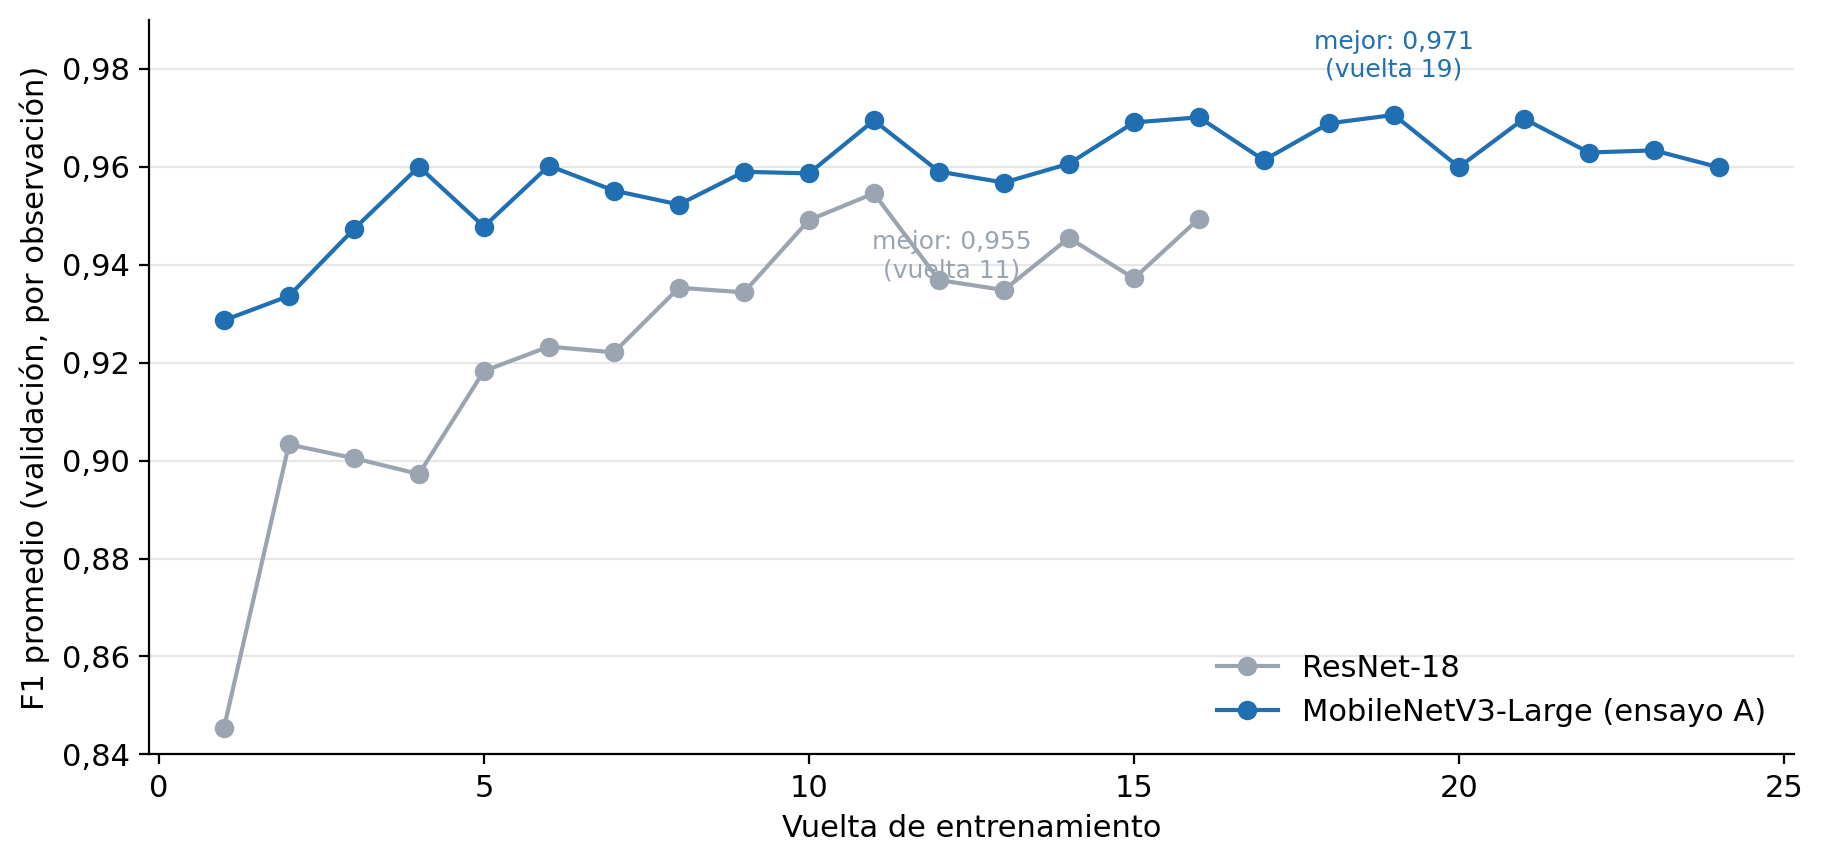
\includegraphics[width=0.92\textwidth]{s5_s6_training_curves.png}
\caption{Resultado en validación después de cada vuelta (\code{runs/*/history.csv}).}
\end{figure}

\begin{table}[H]
\centering
\small
\begin{tabularx}{\textwidth}{Y R R}
\toprule
\textbf{Medida (validación)} & \textbf{ResNet-18} & \textbf{MobileNet A}\\
\midrule
F1 promedio por observación & 0,954 & \textbf{0,971}\\
F1 promedio por foto        & 0,900 & \textbf{0,925}\\
Aciertos por observación    & 95,9\,\% & \textbf{98,0\,\%}\\
\bottomrule
\end{tabularx}
\end{table}

\subsection{Qué falta de la Semana 5}

\begin{itemize}[leftmargin=*]
    \item Evaluar el ensayo A una sola vez en la prueba. Hasta entonces MobileNet
    no tiene resultado de prueba.
    \item Medir tamaño y tiempo en un celular Android real.
\end{itemize}

% =========================================================
\section{Semana 6: resultados por nivel taxonómico}
% =========================================================

\subsection{Taxonomía usada}

La familia, el orden, la clase y el filo de cada género se tomaron de los datos
originales de FungiTastic, sin cambios. Se comprobó que las 25\,290 observaciones
los tienen completos y que ningún género aparece con dos familias distintas.

\begin{table}[H]
\centering
\small
\begin{tabularx}{\textwidth}{l Y Y Y l r}
\toprule
\textbf{Género} & \textbf{Familia} & \textbf{Orden} & \textbf{Clase} & \textbf{Filo} & \textbf{Especies}\\
\midrule
\textit{Amanita}     & Amanitaceae     & Agaricales     & Agaricomycetes  & Basidiomycota & 19\\
\textit{Auricularia} & Auriculariaceae & Auriculariales & Agaricomycetes  & Basidiomycota & 2\\
\textit{Ganoderma}   & Polyporaceae    & Polyporales    & Agaricomycetes  & Basidiomycota & 5\\
\textit{Geastrum}    & Geastraceae     & Geastrales     & Agaricomycetes  & Basidiomycota & 9\\
\textit{Hericium}    & Hericiaceae     & Russulales     & Agaricomycetes  & Basidiomycota & 3\\
\textit{Lycoperdon}  & Lycoperdaceae   & Agaricales     & Agaricomycetes  & Basidiomycota & 10\\
\textit{Morchella}   & Morchellaceae   & Pezizales      & Pezizomycetes   & Ascomycota    & 3\\
\textit{Pleurotus}   & Pleurotaceae    & Agaricales     & Agaricomycetes  & Basidiomycota & 3\\
\textit{Trametes}    & Polyporaceae    & Polyporales    & Agaricomycetes  & Basidiomycota & 7\\
\textit{Xylaria}     & Xylariaceae     & Xylariales     & Sordariomycetes & Ascomycota    & 5\\
\bottomrule
\end{tabularx}
\end{table}

En total son 10 géneros, 9 familias, 7 órdenes, 3 clases y 2 filos.

\subsection{Cómo se mide}

El modelo solo nombra géneros. Para otro nivel se toma el género que eligió y se
mira su familia, orden, etc. Ejemplo: si la foto es \textit{Ganoderma} y el
modelo dice \textit{Trametes}, falla el género pero acierta la familia, porque
ambos son Polyporaceae. No se entrenó nada nuevo: se usaron las respuestas ya
guardadas de cada modelo.

\subsection{Resultados}

F1 promedio por observación. Entre corchetes, el rango donde probablemente está
el valor real (95\,\%).

\begin{table}[H]
\centering
\small
\begin{tabularx}{\textwidth}{l l R R R R R}
\toprule
\textbf{Modelo} & \textbf{Partición} & \textbf{Género} & \textbf{Familia} & \textbf{Orden} & \textbf{Clase} & \textbf{Filo}\\
\midrule
ResNet-18   & validación & 0,954 & 0,959 & 0,962 & 0,987 & 0,981\\
ResNet-18   & prueba     & 0,946 & 0,950 & 0,952 & 0,961 & 0,968\\
MobileNet A & validación & 0,971 & 0,972 & 0,971 & 0,979 & 0,992\\
\bottomrule
\end{tabularx}
\end{table}

Rangos a nivel de género: ResNet-18 validación [0,945–0,962], prueba
[0,933–0,957]; MobileNet A validación [0,956–0,981].

\begin{itemize}[leftmargin=*]
    \item \textbf{Subir a familia u orden mejora poco.}
    De los 140 errores de ResNet-18 en validación, solo 24 quedan dentro de la
    misma familia y 51 dentro del mismo orden. La mayoría de los errores son entre
    hongos poco emparentados.
    \item \textbf{Las confusiones más comunes} son \textit{Amanita} con
    \textit{Lycoperdon} y \textit{Ganoderma} con \textit{Trametes}.
    \item \textbf{Ascomycota y Basidiomycota casi nunca se confunden}: más del
    99\,\% de aciertos a nivel de filo.
    \item En clase y filo el F1 no siempre sube, porque \textit{Morchella} es sola
    su clase y tiene muy pocas observaciones; un error pesa mucho.
\end{itemize}

\subsection{Especies más difíciles}

Porcentaje de observaciones en las que el modelo acierta el género, para
especies con al menos 5 observaciones que quedan por debajo del 90\,\%:

\begin{table}[H]
\centering
\small
\begin{tabularx}{\textwidth}{Y r r r r}
\toprule
\textbf{Especie} & \textbf{Obs. val.} & \textbf{ResNet-18 val.} & \textbf{MobileNet A val.} & \textbf{ResNet-18 prueba}\\
\midrule
\textit{Auricularia mesenterica} & 7  & 43\,\% & 57\,\% & 62\,\%\\
\textit{Hericium cirrhatum}      & 17 & 76\,\% & 88\,\% & 73\,\%\\
\textit{Trametes cinnabarina}    & 26 & 77\,\% & 96\,\% & 68\,\%\\
\bottomrule
\end{tabularx}
\end{table}

Son especies con pocas fotos y con un aspecto distinto al del resto de su género.
MobileNet mejora en las tres, pero \textit{Auricularia mesenterica} sigue siendo
la más difícil.

% =========================================================
\section{Semana 6: orden del código}
% =========================================================

El programa de entrenamiento era un solo archivo grande. Se separó en partes,
cada una con una tarea: cargar y verificar los datos, preparar las fotos, crear el
modelo, entrenar, evaluar y guardar los resultados
(\code{scripts/train/pipeline/}). Así, en la Fase 5 se podrán añadir los datos de
ubicación y clima cambiando solo la carga de datos y el modelo.

Se comprobó que el código nuevo da \textbf{exactamente los mismos resultados}
que el anterior, incluso al pausar y continuar un entrenamiento, y que los modelos
ya guardados se pueden abrir y continuar. Hay 17 pruebas automáticas y todas
pasan.

% =========================================================
\section{Pendientes}
% =========================================================

Los resultados son de una sola corrida por modelo; las diferencias pequeñas entre
modelos deben tomarse con cautela. Falta:

\begin{enumerate}[leftmargin=*, topsep=0pt]
    \item Evaluar MobileNet (ensayo A) una vez en la prueba y añadirlo a la
    tabla por nivel taxonómico.
    \item Medir el modelo en un celular Android.
    \item Corregir un detalle de configuración de Git en Windows que hace que los
    archivos del dataset parezcan modificados y bloquea el entrenamiento en esa
    computadora.
\end{enumerate}

\end{document}
